\documentclass{standalone}
\usepackage{tikz}
\usepackage{pst-3dplot}
\usetikzlibrary{arrows, shapes, angles, quotes}
\usepackage{amsmath}
\usepackage{bm}
\begin{document}
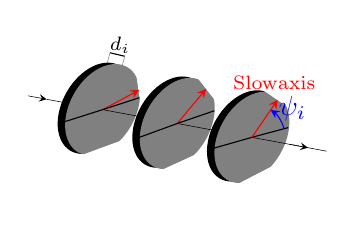
\begin{tikzpicture}[x={(1:1cm)},y={(75:1cm)},z={(190:1cm)}]

    % 1
    \fill[black] (0.9,-0.18) ellipse (0.45 and 0.6);
    \fill[gray] (1,-0.2) ellipse (0.45 and 0.6);
    % base:
    \draw[fill=white, draw=none] (0.5,-0.95)--(1.5,-0.55)--(1.5,-1.15)--(0.5,-1.15)--(0.5,-0.95);
    % print direction:
    \draw[fill=white, draw=none] (1.32,0.41)--(1.45,0.1)--(1.45,-0.1)--(1.32,0.23)--(1.32,0.41);
    
    % 2
    \fill[black] (1.9,-0.38) ellipse (0.45 and 0.6);
    \fill[gray] (2,-0.4) ellipse (0.45 and 0.6);
    % base:
    \draw[fill=white, draw=none] (1.5,-1.25)--(2.5,-0.73)--(2.5,-1.43)--(1.5,-1.43)--(1.5,-1.25);
    % print direction:
    \draw[fill=white, draw=none] (2.1,0.39)--(2.4,0.1)--(2.4,-0.1)--(2.1,0.2)--(2.1,0.39);
    
    % 3
    \fill[black] (2.9,-0.58) ellipse (0.45 and 0.6);
    \fill[gray] (3,-0.6) ellipse (0.45 and 0.6);
    % base:
    \draw[fill=white, draw=none] (2.5,-1.5)--(3.5,-0.9)--(3.5,-1.6)--(2.5,-1.6)--(2.5,-1.5);
    % print direction:
    \draw[fill=white, draw=none] (3,0.21)--(3.5,-0.1)--(3.5,-0.3)--(3,0.01)--(3,0.21);
    
    \node (orig) at (3,-0.6) {};
    \node (printdir) at (3.2,-0.11) {};
    \node (horiz) at (3.43,-0.48) {};
    
    \node[] (b) at (1.0,0.65) {\scriptsize $d_i$};
    \draw[] (0.9,0.55) -- (1.1,0.5);
    \draw[very thin, gray] (0.9,0.55) -- (0.9,0.42);
    \draw[very thin, gray] (1.1,0.5) -- (1.1,0.37);
    
    % 3
    \node[red] (abe) at (3.1,0.11) {\scriptsize Slow \\ axis};
    \draw[] (2.5,-0.75) -- (3,-0.6) -- (3.43,-0.48);
    \draw[->, >=stealth, red] (3,-0.6) -- (3.2,-0.11);
    \pic [draw=blue,text=blue,->,"$\psi_i$", angle radius=12, angle eccentricity=1.5, >=stealth] {angle = horiz--orig--printdir};
    
    % 2
    \draw[->, >=stealth, red] (2,-0.4) -- (2.25,0.05);
    \draw[] (1.5,-0.60) -- (2,-0.4) -- (2.43,-0.24);
    
    % 1
    \draw[->, >=stealth, red] (1,-0.2) -- (1.4,0.05);
    \draw[] (0.5,-0.37) -- (1,-0.2) -- (1.43,-0.05);
    
    \draw[->, >=stealth, very thin] (0,0) -- (0.25,-0.05);
    \draw[very thin] (0.25,-0.05) -- (0.5,-0.1);
    \draw[very thin] (1,-0.2) -- (1.5,-0.3);
    \draw[very thin] (2,-0.4) -- (2.5,-0.5);
    \draw[->, >=stealth, very thin] (3,-0.6) -- (3.75,-0.75);
    \draw[very thin] (3.5,-0.7) -- (4,-0.8);
    
\end{tikzpicture}
\end{document}